\documentclass{exam}
\usepackage{amsmath}
\usepackage{pgfplots}
\usepackage{tikz}
\usepackage{gensymb}
\pgfplotsset{compat=1.15}
\usepackage[margin=0.25in]{geometry}

\begin{document}

\title{Mathematics Mock Exam}
\date{Tag: 99879823}
\maketitle

\section{ARITHMETIC}
\begin{questions}
\question What is the result of $56 + 29$?
\question Calculate the difference between $500$ and $168$.
\question Multiply $17$ by $4$.
\question Divide $81$ by $9$.
\question What is $4$ to the power of $2$?
\end{questions}

\section{NUMBER AND PLACE VALUE}
\begin{questions}
\question Write the number $8972$ in words.
\question What is the value of the digit $7$ in the number $478$?
\question Write $8000 + 900 + 70 + 5$ in standard form.
\question Round the number $8975$ to the nearest thousand.
\question What is the Roman numeral for $100$?
\end{questions}

\section{FRACTIONS}
\begin{questions}
\question Simplify the fraction $\frac{24}{48}$.
\question Add the fractions $\frac{1}{2}$ and $\frac{3}{4}$.
\question Subtract $\frac{3}{5}$ from $\frac{4}{5}$.
\question Multiply $\frac{3}{4}$ by $\frac{2}{3}$.
\question Divide $\frac{3}{5}$ by $\frac{2}{3}$.
\end{questions}

\section{DECIMALS}
\begin{questions}
\question Write $0.625$ as a fraction.
\question Add $3.2$ and $5.78$.
\question Subtract $1.2$ from $4.78$.
\question Multiply $2.3$ by $3.6$.
\question Divide $3.6$ by $0.6$.
\end{questions}

\section{PERCENTAGES}
\begin{questions}
\question Write $55\%$ as a fraction.
\question What is $40\%$ of $250$?
\question Increase $500$ by $20\%$.
\question Decrease $120$ by $30\%$.
\question What percentage of $60$ is $15$?
\end{questions}

\section{MEASUREMENT AND GEOMETRY}
\begin{questions}
\question Calculate the area of a rectangle with length $8$ cm and width $4$ cm.
\question What is the perimeter of a square with side length $5$ cm?
\question Calculate the volume of a cube with edge length $4$ cm.
\question What is the total surface area of a cuboid with dimensions $3$ cm, $4$ cm and $5$ cm?
\question What is the circumference of a circle with a radius of $4$ cm? (Use $\pi \approx 3.14$)
\end{questions}

\section{GRAPHS AND BAR CHARTS}
\begin{questions}
\question The bar chart below shows the number of books read by a group of students in different months. 

\begin{center}
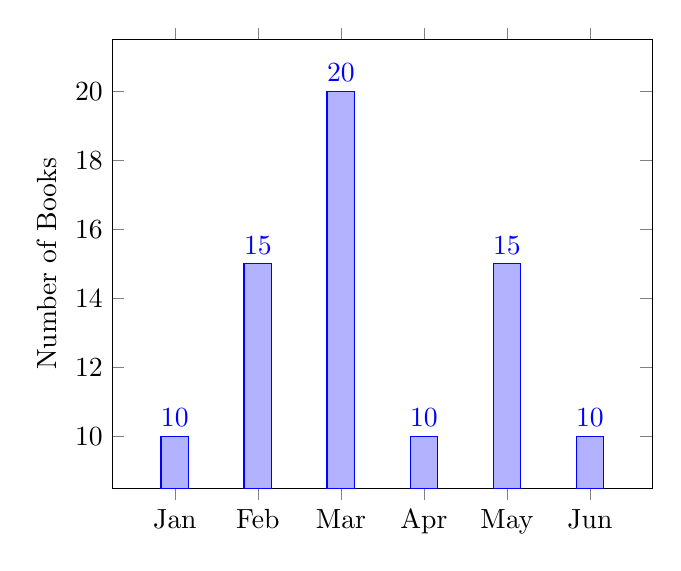
\begin{tikzpicture}
\begin{axis}[
    ybar,
    enlargelimits=0.15,
    ylabel={Number of Books},
    symbolic x coords={Jan, Feb, Mar, Apr, May, Jun},
    xtick=data,
    nodes near coords,
    nodes near coords align={vertical},
]
\addplot coordinates {(Jan,10) (Feb,15) (Mar,20) (Apr,10) (May,15) (Jun,10)};
\end{axis}
\end{tikzpicture}
\end{center}

\begin{parts}
\part Which month did the students read the most books?
\part How many books were read in February?
\part How many more books were read in March compared to June?
\end{parts}

\question The line graph below shows the temperature in a city over a week.

\begin{center}
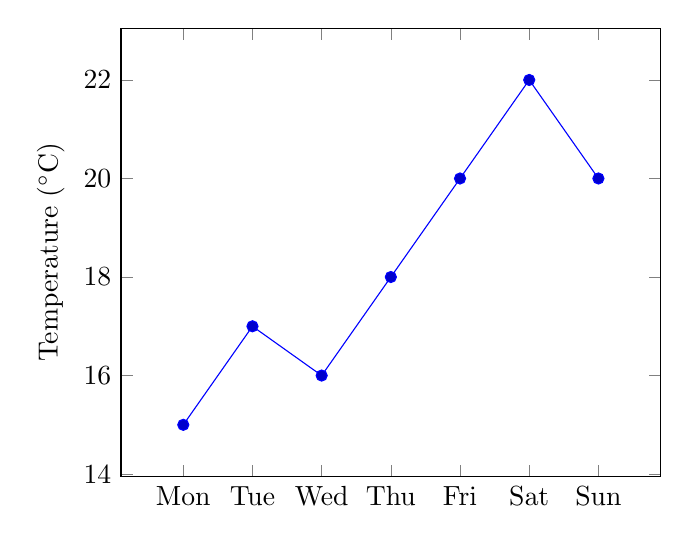
\begin{tikzpicture}
\begin{axis}[
    enlargelimits=0.15,
    ylabel={Temperature (\degree C)},
    symbolic x coords={Mon, Tue, Wed, Thu, Fri, Sat, Sun},
    xtick=data,
]
\addplot coordinates {(Mon,15) (Tue,17) (Wed,16) (Thu,18) (Fri,20) (Sat,22) (Sun,20)};
\end{axis}
\end{tikzpicture}
\end{center}

\begin{parts}
\part On which day was the temperature the highest?
\part What was the temperature on Wednesday?
\part Did the temperature rise or fall from Tuesday to Wednesday?
\end{parts}
\end{questions}

\end{document}
